\chapter{The Booster Neutrino Beam}\label{ch:beam}


The MicroBooNE detector is stationed at Fermi National Accelerator Laboratory (FNAL) where it receives neutrinos from both the Booster Neutrino Beam (BNB) and Neutrinos from the Main Injector (NuMI) beams. MicroBooNE is on-axis for the BNB and off-axis by 135 mrad for NuMI. For the purpose of this analysis, only data from the BNB was used. This chapter will discuss how neutrinos are created using the BNB. How these neutrinos are produced as well as their flux through the MicroBooNE detector is necessary for any analysis, for example, the neutrino production process can help to identify sources of systematic uncertainties. 

The BNB is a very pure $\nu_{\mu}$ beam, with only 0.6\% contamination from $\nu_{e}s$. The energy also peaks around 700 MeV which is desired based on the probability of oscillation equation which depends on the the value of $L/E$, where $L$ is the distance of the detector from the neutrino beam and $E$ is the energy of the neutrino beam. $L/E$ was chosen to increase the probability of seeing neutrino oscillations in the MiniBooNE Low Energy Excess (LEE) range based on the probability of oscillation equation, which is $ P_{\nu_{\mu}\rightarrow \nu_{e}}\left(L,E\right) = \sin^2 2\theta \sin^2 \left(1.27\Delta m^2 \frac{L}{E_{\nu}}\right)$. The BNB collides 8.9 GeV/c momentum protons from the FNAL booster synchrotron into a beryllium target which produces a high flux of neutrinos. The protons originate from $H^2$ gas molecules that are turned into $H^-$ ions by a Cockroft-Walton generator shown in figure \ref{fig:generator}. The $H^-$  





\begin{figure}[htp!]
\centering
	\begin{subfigure}[b]{.4\textwidth}
	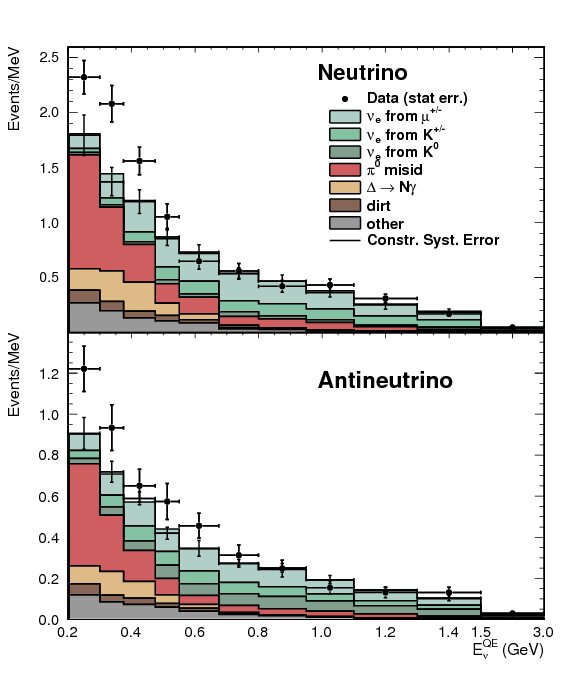
\includegraphics[width=\textwidth]{figs/lee.png}
	\caption{Low Energy excess seen in MiniBooNE}
	\label{fig:lee}
	\end{subfigure}
	\quad
	\begin{subfigure}[b]{.4\textwidth}
	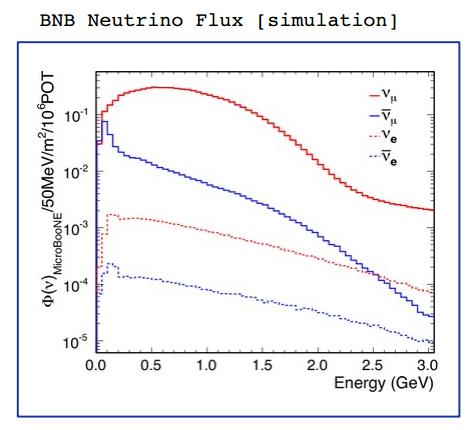
\includegraphics[width=\textwidth]{figs/bnbflux.png}
	\caption{Energy spectrum of the Booster Neutrino Beam at Fermi National Laboratories}
	\label{fig:bnbflux}
	\end{subfigure}
	\quad
\label{fig:figures}
\caption{\ref{fig:bnbflux} Flux of BNB at FNAL.}
\end{figure}
